\subsection{Personalized Denoiser}

\subsubsection{Motivation}
The Denoiser model \cite{defossez2020} offers raw waveform speech enhancement using an encoder-decoder architecture with a U-Net structure.
Altough the model great performance, it lacks the ability to personalize the enhancement process.
To introduce personalization, we propose a personalized denoiser model or simply PDenoiser. PDernoiser consists of two major modules: a speaker embedding module and a denoising module.
The speaker embedding module is responsible for extracting speaker-specific features from the input speech signal, while the denoising module is responsible for enhancing the speech signal based on the extracted speaker features.
The architecture of the PDenoiser model is shown in Figure \ref{fig:pdenoiser-architecture}.

\begin{figure}[ht]
    \centering
    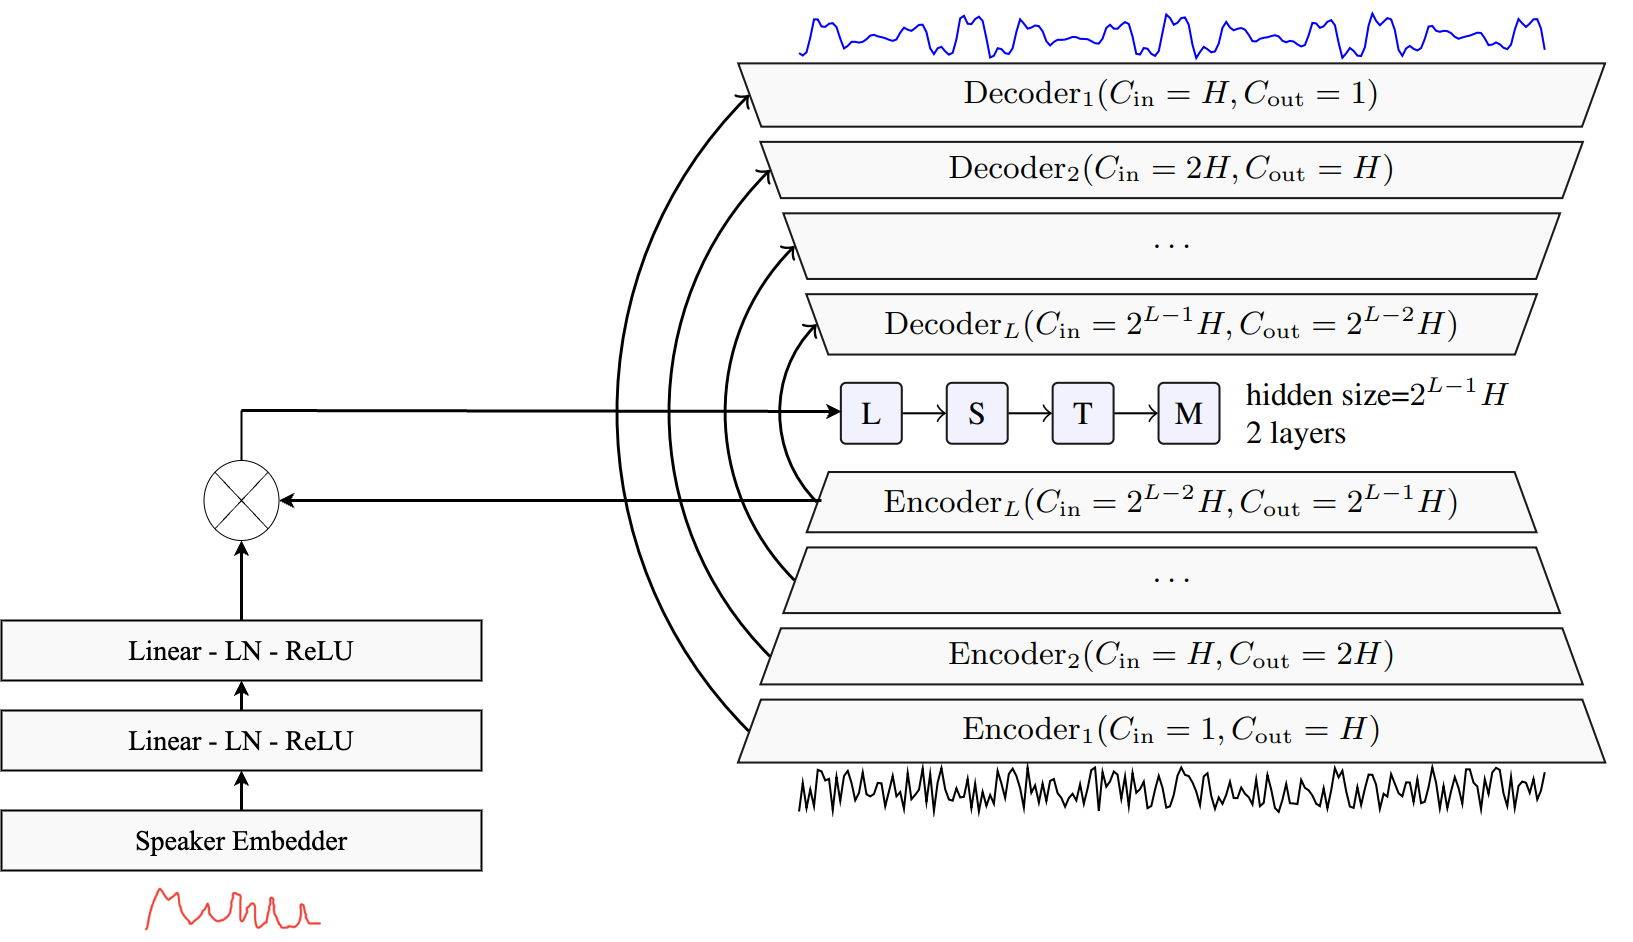
\includegraphics[width=0.8\textwidth]{images/experiments/pdenoiser/pdenoiser-arch.png}
    \caption{PDenoiser Architecture}
    \label{fig:pdenoiser-architecture}
\end{figure}

\subsubsection{Speaker Embedding Module}
We propose two different variations of the speaker embedding module: a TitaNet-based speaker embedding module and a ECAPA-TDNN-based speaker embedding module.
Both speaker embedders output a fixed-sized speaker embedding of size 192.
This speaker embedding is then passed to a repeated 2 times block that consists of: a linear layer followed by a layer normalization and a ReLU activation function.
The previous block is used to increase the dimensionality of the speaker embedding to 512.

\subsubsection{Denoising Module}
The denoising module is a regular Denoiser model with the output of last encoder layer scaled by the output of speaker embedding module just before the LSTM.

\subsubsection{Experimental Setup}
We trained the PDenoiser model on the training set of our dataset for 33 epochs for  with a batch size of 58 per GPU. We trained the model using Kaggle's 2 NVIDIA Tesla T4 GPUs.
The noisy audio clips were generated on the fly by mixing speakerA and speakerB clean audio clips. The SNR of the noisy audio clips was randomly selected from values of 0, 3, 6, 10, 20.
The clean audio clips were cropped to 3 seconds before mixing as an augmentation technique. The audio clips were sampled at 16kHz.
The Adam optimizer was used with a learning rate of $1 \times 10^{-4}$ with Cosine Annealing and beta values of 0.9 and 0.999. Model exponential moving average (EMA) was used with a decay of 0.999.
We employed a mixture of loss functions, including L1 loss, Multi Resolution STFT loss and TAP loss with weights 1, 0.4 and 0.3 respectively.
Both speaker embedding module pretrained variation were frozen during the training of the PDenoiser model.

\subsubsection{Results}
Waiting for gadwal to add results.
% We tested the model on two test sets: personalized DNS blind test set and the test set of our dataset. Results are show in table \ref{tab:pffsn-dns} and \ref{tab:pffsn-our}.


\subsubsection{Limitations}
Upon listening to the outputs of the PDenoiser model on our dataset we noticed that it struggles in different scenarios:
\begin{itemize}
    \item When the primary speaker tone changes i.e, when the speaker is angry, happy, sad, etc.
    \item The interfering speaker when the primary speaker and the interfering speaker are speaking at the same time.
    \item Both infering and primary speaker have close audio loudness.
    \item Both infering and primary speaker have close audio frequency.
\end{itemize}